\chapter{Assembling programming environment}

% SPI wire programming

\subsection{Bug and limitations}

% connected to TOS build

\section{Mspdebug}

\section{Printf library}
\label{sec:printf_library}

When a code is first written, more often than not, it does not work as
expected. Unit testing helps, but often errors arise from making false
assumptions and these may be reflected in tests as well. In such case,
only observing the actual behaviour during execution will lead to
fixing the issue.

But how to observe the behaviour of a wireless sensor node after it
has been flashed with a new executable image?

One way is to observe LEDs on the circuit board.  In case of the
chronos watch, which has no LEDs, LCD display can be used instead, to
even better results. But only small amount of information can be
retrieved through through such a channel. Another possibility is to
use mspdebug tool mentioned before.  However if you ask a computer
programmer which tool he most commonly uses to find out what's
happening in his program, \emph{the debugger} will be his second
answer. The first would be \emph{printf}.

TinyOS has a convenient printf library that allows sending text
messages from running device to the PC and display them in a console.
Its use is simple and comprises of following steps:

\begin{itemize}
  \item Include the printf library files to the build, by adding
    following line to your Makefile:

    \texttt{CFLAGS += -I\$(TOSDIR)/lib/printf}

  \item Optionally, increase the printf buffer size (250 bytes by
    default), by adding following line to your Makefile:

    \texttt{CFLAGS += -DPRINTF\_BUFFER\_SIZE=<NEW\_SIZE>}

  \item Instantiate printf components in your application
    configuration. This step depends on which implementation of
    printf you use. See following sections for details.

  \item Add following include in the file you wish to use printf in:

    \texttt{\#include ``printf.h''}

  \item Use \texttt{printf} statement to display messages and
    occasionally \texttt{printfflush} to ensure that they are not stuck
    in a buffer.

    \texttt{printf(``Value is \%d\textbackslash n'', value);} \\
    \texttt{printfflush();}

  \item To receive the messages you will need to run the printf
    client. How this is done also depends on which implementation of
    print you use.
\end{itemize}

Now before we delve in to the specific implementations there's a warning
regarding printf buffering. Only after the buffer is filled or when
you call \texttt{printfflush} does the data get actually sent to the
PC. This isn't however immediate. If you very quickly print more text
than the capacity of the buffer, some of the messages will be lost!
Also note that \texttt{printfflush} is non-blocking and after calling
it, the buffer may still be full for a while, and thus messages
may still get lost.

To overcome this,  you can shorten your messages, slow down printing
rate to ensure enough time to transmit current contents of the buffer
or increase the size of the buffer.

\subsection{Mspdebug printf}

\subsection{Radio printf}

\subsection{Serial port printf}
Third version of the printf library uses the serial port connection to
communicate with the PC. On the watch end it uses the UART (Universal
Asynchronous Receiver/Transmitter) hardware driver. This has both
serious advantages and a disadvantage.

Main advantage is, that serial communication is most reliable and best
supported way of sending printf messages in TinyOS. For example the
PrintfClient tool that comes with vanilla TinyOS, handles receiving
the packets and displaying them in the console. Also it is the least
intrusive one, since it neither requires halting the MCU nor sending
packets through the radio transceiver.

Main drawback however is that Texas Instruments did not make the UART
pins easily accessible on the chronos circuit board and certain
hardware modification is necessary to reach them. How to perform it,
is described in Appendix \ref{appendix:uart_pins}. Fortunately, no
additional hardware besides the USB debug interface is necessary after
the modification is done.

To enable this version of printf library you need to augment
instructions given in section \ref{sec:printf_library} with following
steps:

\begin{itemize}
  \item Instantiate these components in your application configuration:

  \texttt{components PrintfC, SerialStartC;}

  \item Connect the watch with hardware modification described in
    Appendix \ref{appendix:uart_pins} to the USB debug dongle and
    connect the dongle to the PC.

  \item To receive messages run PrintfClient:

  \texttt{java net.tinyos.tools.PrintfClient -comm serial@/dev/ttyACM0:chronos}

  Note that watch may have shown in \texttt{\textbackslash dev} under
  different name, most commonly
  \texttt{\textbackslash dev\textbackslash ttyACM1}
\end{itemize}

\section{Eclipse integrated development environment}

The most practical way to work with TinyOS code is using the Eclipse
IDE. Some great work has been done on that field, resulting in the Yeti 2
plugin. It supports TinyOS application and platform development,
providing many features. Below we'll describe the most important ones.

Firstly, in editor, there is some very good {\bf code completion} available
which eases writing both module and configuration files. It completes
component instantiations and connections. Also it completes interface
calls, function calls and variable names, and after adding a
\texttt{uses} or \texttt{provides} declaration, it offers to create
command and event stubs. These features are best shown on the
following series of Figures, \ref{fig:first_compl} through
\ref{fig:last_compl}.

\begin{figure}[h]
  \centering
  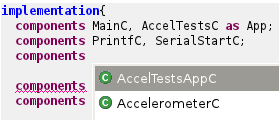
\includegraphics[width=0.85\textwidth]{img/eclipse_compl1.png}
  \caption{Component instantiation completion.}
  \label{fig:first_compl}
\end{figure}

\begin{figure}[h]
  \centering
  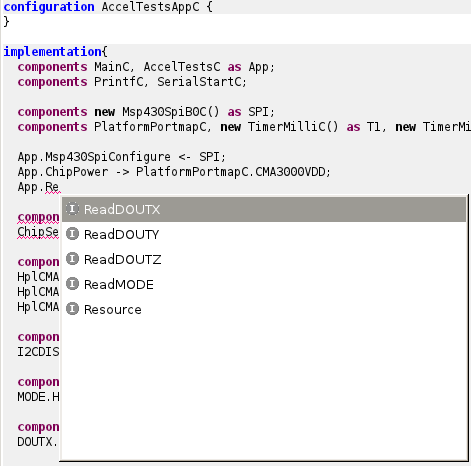
\includegraphics[width=0.8\textwidth]{img/eclipse_compl2.png}
  \caption{User connection completion.}
\end{figure}

\begin{figure}[h]
  \centering
  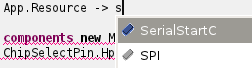
\includegraphics[width=0.9\textwidth]{img/eclipse_compl3.png}
  \caption{Provider connection completion.}
\end{figure}

\begin{figure}[h]
  \centering
  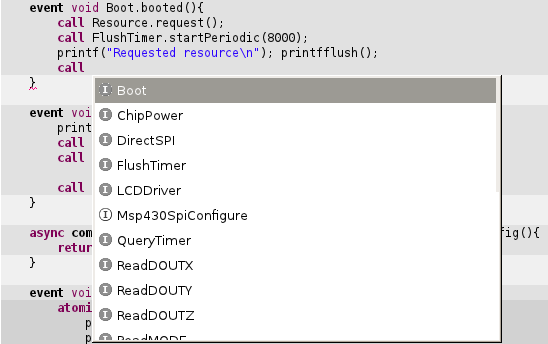
\includegraphics[width=0.9\textwidth]{img/eclipse_compl4.png}
  \caption{Interface completion.}
\end{figure}

\begin{figure}[h]
  \centering
  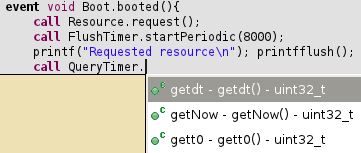
\includegraphics[width=0.9\textwidth]{img/eclipse_compl5.png}
  \caption{Command completion.}
\end{figure}

\begin{figure}[h]
  \centering
  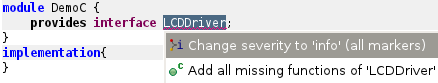
\includegraphics[width=0.9\textwidth]{img/eclipse_compl6.png}
  \caption{Command stubs generation.}
  \label{fig:last_compl}
\end{figure}

Another very useful feature, especially for a new developer wishing to
familiarize himself with TinyOS structure is the {\bf component
explorer}. It graphically displays components instantiated and
interconnected in configurations. Interfaces can be viewed as well.
Starting at the top level application configuration, every part of
it's code can be reached. This is by far the most efficient way to
explore the call hierarchy and find where particular functions are
implemented. Example of the PrintfC configuration, viewed through
the component explorer is shown in figure
\ref{fig:eclipse_compexp}.

\begin{figure}[h]
  \centering
  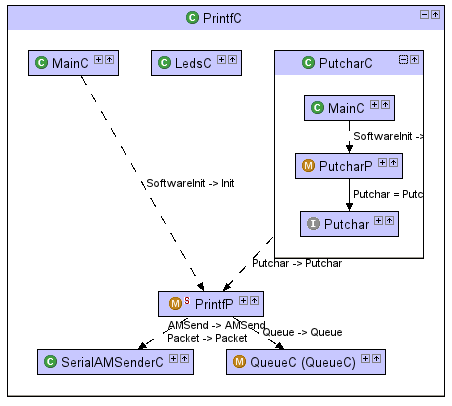
\includegraphics[width=0.7\textwidth]{img/eclipse_compexp.png}
  \caption{Component explorer showing PrintfC configuration.}
  \label{fig:eclipse_compexp}
\end{figure}

The eclipse editor also gives many warnings about the code without
triggering compilation. Moreover many of these useful warnings are not
raised by NesC compiler, which is an added value. 

Finally, one of the most useful parts of Yeti 2 is {\bf the debugger}.
The chain of tool invocations, needed to debug an application on the
chronos watch is long, but running them is as easy as pressing a
button in the IDE. At the lowest level, the \emph{mspdebug}
communicates with the watch through the USB debugging dongle. It runs
a GDB Server to which newer versions of \emph{msp430-gdb} are able to
connect. Eclipse runs this last executable and forms practical data
views, reading crude data from GDB. Here is a list of most useful
views and features:
\begin{itemize}
  \item Single stepping through code in NesC editor.
  \item Call stack view.
  \item Breakpoints list (though limited to 3 active at any moment).
  \item Disassembly view.
  \item Raw memory view.
  \item Registers view.
  \item Local variables view.
  \item Module variables view.
\end{itemize}

Yetti 2 provides many more functions not mentioned here, most of which
are standard to Eclipse IDE and expected to be available for any
supported programming language. Developer naturally explores them
while using the IDE.

The installation is described in Appendix \ref{appendix:env_install}
and a preconfigured setup is available in the virtual machine
distributed with this work.

\section{Console centric development}

It is also possible to develop TinyOS code without using any
IDE\footnote{In fact, this is exactly how TinyOS was first written.}.
To support such style of development two changes were necessary.
Firstly, the environment variables were configured to point to the
TinyOS source code locations and Makefile rules. This makes it
possible to use make command to build applications. Secondly, syntax
and indentation configurations files for vim were added to ensure
convenient and practical code editing.  Having both working make and
good text editor allows for development almost as efficient as with
the Eclipse IDE. The only setback is that if the developer is not
familiar with TinyOS naming, he will not receive aid from code
completion.

\section{Development virtual machine}

The setup of all the tools needed to work on the TinyOS Chronos
platform and application code, is complicated and takes time. To ease
this step for new developers, a virtual machine image was created.
All the tools have been installed in it and configured, to work
out-of-box. The most recent version of the source code is checked out
and imported into Eclipse IDE, with a run configuration ready to build
and install TinyOS Blink application.  All that is left to the user,
is connecting the watch through the USB debug interface and pressing
Run button.

% Vim settings:
% vim: set textwidth=70:
% vim: set fo+=t:
